% !TEX root = template.tex

\section{Processing Pipeline}
\label{sec:processing_architecture}
The project can be divided in 3 parts: the dataset creation, the neural network creation and the benchmark prediction.
In order to make an action recognition model it was firstly created a proper dataset. All the signals were divided in several overlapping windows and were thrown into a \gls{cnn} made up with convolutional layers and fully connected layers.
When the neural network was trained and tested, 

\MC{(SISTEMA)
- DRAW A DIAGRAM OF THE PIPELINE
- DESCRIPTION OF THE GENERAL APPROACH}

\section{Signals and Dataset}
\label{sec:model}

\subsection{Measurement setup}
The signals we have worked on were provided by DLR official website \cite{DLR}. We took into considerations two of the three published Matlab datasets: \textit{ARS\_DLR\_Data\_Set\_V2.mat} and \textit{ARS\_DLR\_Benchmark\_Data\_Set.mat}. 
Both of them are made up of signals recovered by a \gls{mems} based \gls{imu} composed by an accelerometer, a gyroscope and a magnetometer. These measurements systems provide informations about the intertial acceleration, the angular velocity and the magnetic field direction.
At the experiment joined fourteen people and the \gls{imu}, that was positioned over the pelvic region of each one (\fig{fig:IMU}), recovered signals during some ordinary motion activities like \textit{standing}, \textit{sitting}, \textit{running}, \textit{jumping}, \textit{lying} and all the trasitional phases from an activity to another.

\begin{figure}
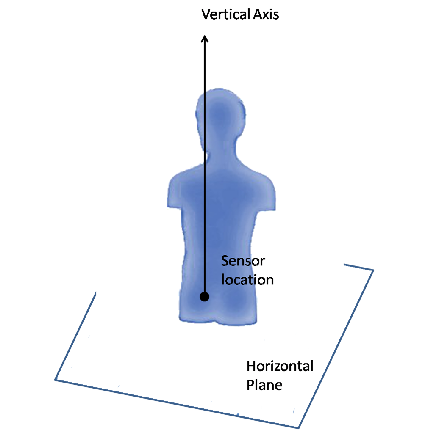
\includegraphics[scale=1.2]{IMU_sensor.pdf}
\caption{Sensor position and the representation of the local frame}
\label{fig:IMU}
\end{figure}

The considered datasets are divided only because they have to be used in different ways, but they are going to be described in the same way according to their identity.

Both datasets are divided in activity sessions, each session is a structure in turn (a sua volta) that contains: a matrix of 10 column in which the first column represents the time domain and the other ones represents the \gls{imu} records over the three local coordinate, a rotation matrix that has the same dimension of the first one that permits to turn to the global frame the first matrix, a vector that contains the activity labels performed during the session and lastly a vector that indicates when each activity starts and ends.

\subsection{Signal pre-processing}
The first pre-processing applied to the dataset consisted in representing the signals according to the global frame
\MC{FROM LOCAL TO GLOBAL FRAME: (MANCA)}


The dataset considered already contains pre-processed data, sampled with T = 0.01 s. In \fig{fig:acc}, \fig{fig:gyr} and \fig{fig:mag} is showed one of the Susanna activity sessions. These figures represent the norm of accelerometer, gyroscope and magnetometer over the three global coordinats insead of three figures for each measurement system. This is only a convenient choose according to the visual meaningfulness of the norm.
From these figures emerges that the mean of angular velocity and the magnetic field swings around zero, on the other hand the acceleration mean shifts near 9.8 m/s according to the gravitational constant value \textit{g}.

It also emerges in each of these figures how the transitorial activities from standing to sitting and vice versa can be observable due to the drastic change of the signals.

\begin{figure}
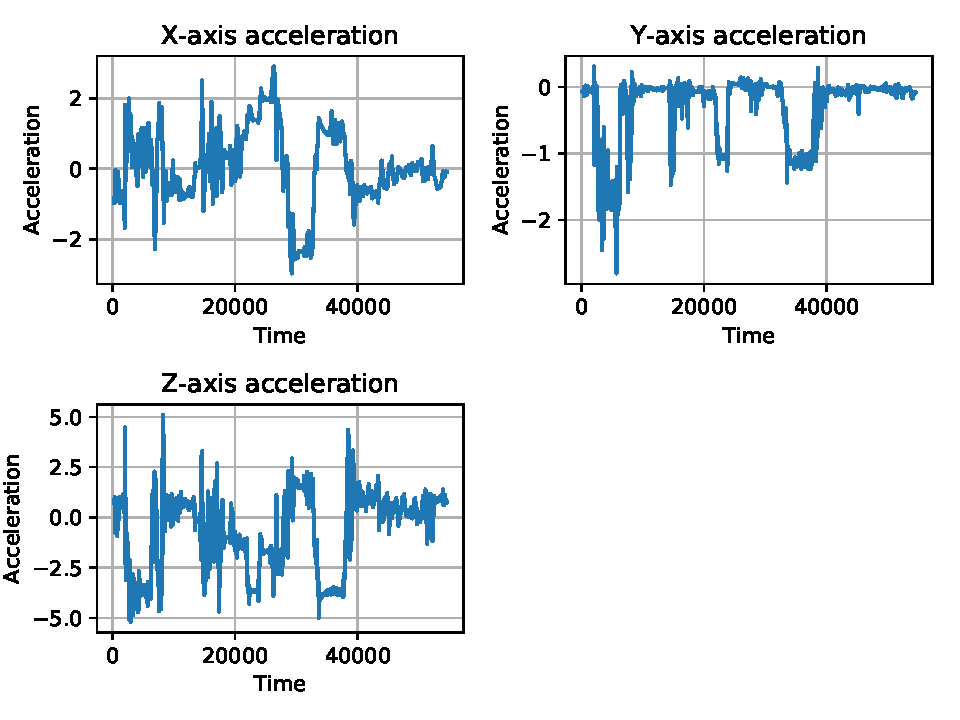
\includegraphics[scale=0.55]{acceleration_susanna.pdf}
\caption{}
\label{fig:acc}
\end{figure}

\begin{figure}
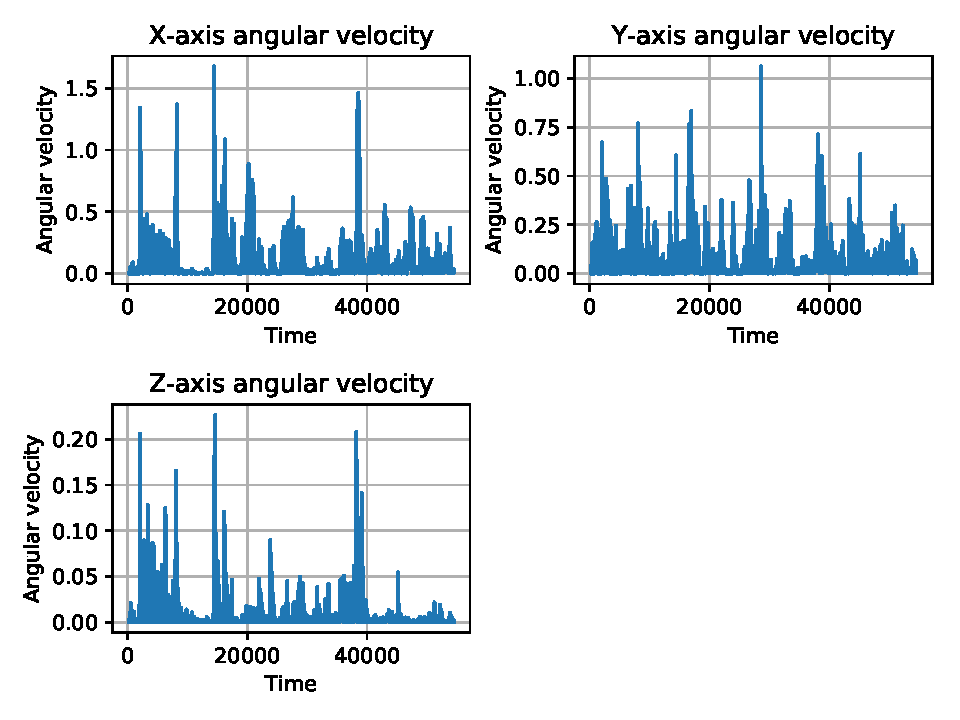
\includegraphics[scale=0.55]{angular_velocity_susanna.pdf}
\caption{}
\label{fig:gyr}
\end{figure}

\begin{figure}
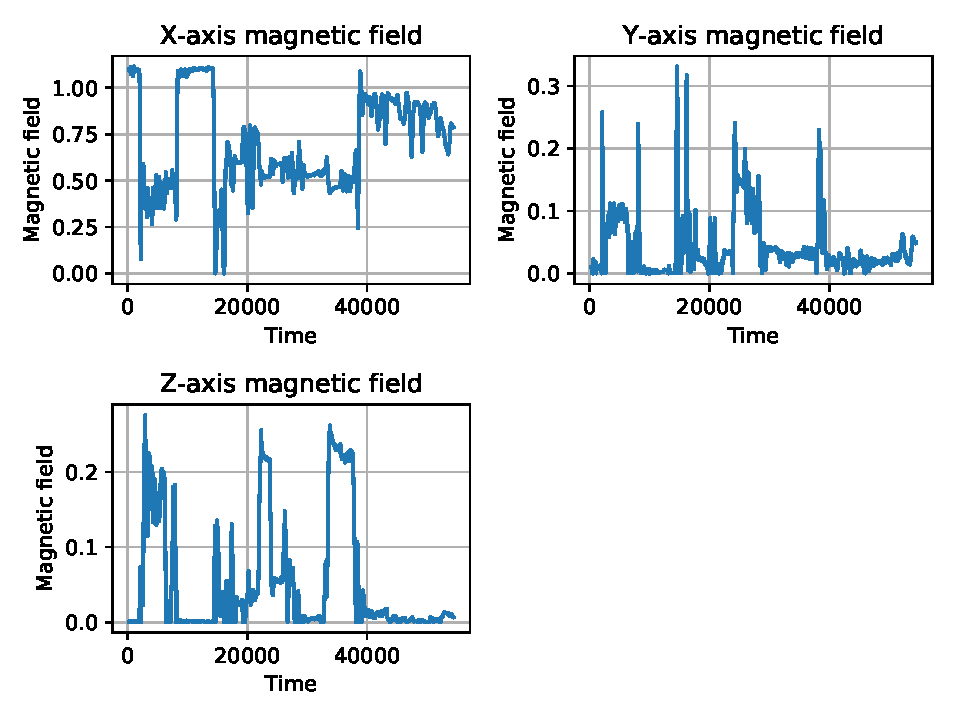
\includegraphics[scale=0.55]{magnetic_field_susanna.pdf}
\caption{}
\label{fig:mag}
\end{figure}


Another sort of pre-processing was made in order to fix the activity indexing of some recordings. It frequently happened to find that, considering two adjacent motion activities, the end of the previous activity and the beginning of the succeeding one were not temporarily neighboring. It happened also to find two activities temporarily overlapping: the end of the previous activity was indexed after the beginning of the second one. 
The authors resolved the problem removing the non indexed data and the data whose label was uncertain so as to not train the \gls{ann} with wrongly labeled data.

Each session is finally represened by a long and straight matrix with nine columns (three for each measurement system) and a number of rows equals to the session duration. Due to the straight sampling time the number of rows stands at around \MR{MILLE!!(find that number)} order of magnitude. Even if motion signals are not two dimensional signals, the pecularity of input shape makes it suitable to be treaten as a kind of image. Therefore according to the adopted strategy of \textit{Gadaleta et al.}, the dataset was processed in order to be fit into a \gls{cnn} \cite{Gadaleta-2018}.


Since the \gls{cnn} needs a fixed input the authors decided to divide in patterns each session matrix and associate to them the corresponding label. The pattern lenght was decided equal to the shortest activity lenght in the whole dataset.

\MC{
-how the patterns were token\\
-transitional pattern are not token\\
-TRANST label is counted in README but no transit pttern appear in the dataset\\
-TRANSIT data in the dataset->yes or no\\
-\tab{tab:label}
}


\begin{table}[b]
\small
	\centering
		\renewcommand{\arraystretch}{1}% Tighter
	\begin{tabular}{@{}lll@{}}
	\toprule
	Label & Index & Description\\ \midrule
	'RUNNING' & $0$ & running \\
	'WALKING' & $1$ & walking \\
	'JUMPING' & $2$ & jumping  \\
	'STNDING' & $3$ & standing \\ 
	'SITTING' & $4$ & sitting\\
	'XLYINGX' & $5$ & lying \\
	'FALLING' & $6$ & falling \\
	'TRANSUP' & $7$ & getting up i.e.: from sitting to standing \\
	'TRANSDW' & $8$ & going down i.e.: from standing to sitting\\
	'TRNSACC' & $9$ & accelerating\\
	'TRNSDCC' & $10$ & deccelerating\\
	'TRANSIT' & $11$ & other transition or irrelevant information\\
	\bottomrule
	\end{tabular}
	\caption{Activities took into consideration with the associated labels}
	\label{tab:label}
\end{table}



\section{Learning Framework}
\label{sec:learning_framework}

\MR{Here you finally describe the learning strategy / algorithm that you conceived and used to solve the problem at stake. A good diagram to exemplify how learning is carried out is often very useful. In this section, you should describe the learning model, its parameters, any optimization over a given parameter set, etc. You can organize this section in \mbox{sub-sections}. You are free to choose the most appropriate structure.}






